\section{Results and discussion}
% Define a custom command to create sections with shared structure

As explained in \ref{sec:methodo}, the first objective is to effectively post-process a single NWP forecast model, by benchmarking the models altogether. 

The following step will be to look at the results in the details to prove the true effectiveness of the post-processing.
\subsection{Post-processing of a single forecasting NWP model}
\subsubsection{Study of the models altogether} 
\paragraph{MAE}
\begin{figure}[htb!]
    \centering
    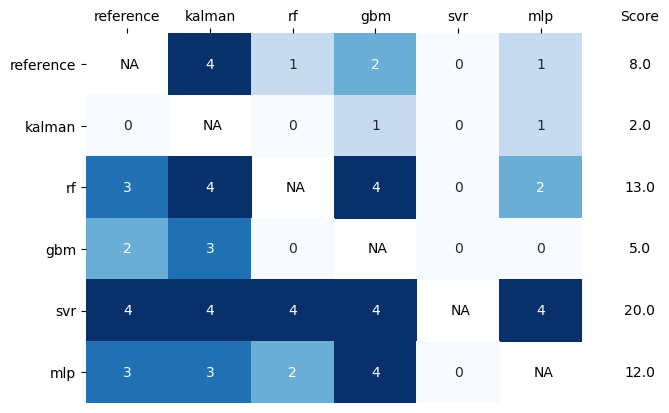
\includegraphics[width=\textwidth]{figures/first_study/significance_matrix_mae.png}
\caption{Significance matrix for MAE. The value $V_{(i,j)}$ of the $(i,j)$ cell indicates how often the model of line i performs better than the one of column j, across the 
4 sites. For example, the MAE of the MLP model post-processed data is 3 times lower than the MAE of the reference model, and for 1 site (4 - 3 = 1), it is higher.}
\end{figure}

\begin{figure}[htb!]
    \centering
    \includesvg[width=0.75\columnwidth]{figures/first_study/comp_for_models_ss_mae.svg}

    \caption{MAE skill score plot across the 4 sites.}
\end{figure}
\paragraph{RMSE}

\subsubsection{Detailled study of the most performing model ()}
\subsection{Benchmarking the linear regression models}
\subsection{Showcase of the hybrid model}